\chapter{Marco teórico}

\section{Desde las ecuaciones de Maxwell a propagación de la luz en guías de onda dieléctricas}

Esta tesis estudia el comportamiento de luz láser de baja potencia (1 mW de potencia de salida) propagada en guías de onda dieléctricas escritas dentro de una muestra de borosilicato. Es por ello que se supone un medio lineal no magnético sin fuentes de carga y de corriente libres. Las ecuaciones de Maxwell (SI) en este régimen son:
\begin{align}
	\nabla\cdot\textbf{D} &= 0, \label{eqn:gauss}
	\\	
	\nabla\times\textbf{E} &= -\frac{\partial \textbf{B}}{\partial t}, \label{eqn:faraday-lenz}
	\\	
	\nabla\cdot\textbf{B} &= 0, \label{eqn:div0}
	\\	
	\nabla\times\textbf{H} &= \frac{\partial \textbf{D}}{\partial t}, \label{eqn:ampere-maxwell}
\end{align}
donde \textbf{E}, \textbf{B}, $\textbf{D}=\varepsilon(\textbf{r})\textbf{E}$ y $\textbf{H}=\textbf{B}/\mu_0$ son los campos eléctrico, campo de densidad de flujo magnético, campo desplazamiento eléctrico y campo magnético, respectivamente. Las guías de onda son invariantes en la dirección de propagación $z$, por lo que el índice de refracción $n=\sqrt{\varepsilon/\varepsilon_0}$ dependerá de las coordenadas transversales al eje óptico, es decir, $n \equiv n(x,y) = n_0 + \Delta n(x,y)$, con $n_0=1.47$ el índice de refracción del borosilicato y $\Delta n \sim 10^{-5}-10^{-3}$ el contraste de las guías de onda.

Aplicando rotor por la izquierda a la ecuación de Faraday-Lenz (\ref{eqn:faraday-lenz}), usando la ecuación de Ampère-Maxwell (\ref{eqn:ampere-maxwell}) y asumiendo una solución temporal harmónica proporcional a $e^{-i\omega t}$ se tiene:

\begin{align}
	\nabla\times\nabla\times\textbf{E} &= -\frac{\partial}{\partial t}(\nabla\times\textbf{B}) = -\frac{\partial}{\partial t}\left(\mu_0\frac{\partial \textbf{D}}{\partial t}\right) = -\frac{n^2}{c^2}\frac{\partial^2 \textbf{E}}{\partial t^2} = n^2k_0^2 \textbf{E}, \label{eqn:rotordoble}
\end{align}
donde $k_0 \equiv \omega/c$ es el número de onda en el vacío. Notemos que, por identidad de cálculo vectorial, se tiene que $\nabla\times\nabla\times\textbf{E} = \nabla(\nabla\cdot\textbf{E}) - \nabla^2\textbf{E}$, y usando la ley de Gauss (\ref{eqn:gauss}) se deduce que $\nabla\cdot \textbf{E} = -\frac{\nabla n^2}{n^2}\cdot\textbf{E}$. Con esto, se obtiene la ecuación 
\begin{equation}
	\left(\nabla^2  + k_0^2n^2\right)\textbf{E} = -\nabla\left( \frac{\nabla n^2}{n^2} \cdot \textbf{E}  \right). \label{eqn:helmholz}
\end{equation}
Análogamente para \textbf{H}, es posible aplicar rotor a la ecuación de Ampère-Maxwell (\ref{eqn:ampere-maxwell}) y usar la ecuación de Faraday-Lenz (\ref{eqn:faraday-lenz}) en conjunto con la divergencia nula de \textbf{B} (\ref{eqn:div0}) y por consiguiente de \textbf{H}:
\begin{align}
	\nabla\times\nabla\times \textbf{H} &= -i \omega \nabla\times\left(\epsilon_0 n^2 \textbf{E}\right) = -i\omega \epsilon_0  \left(n^2 \nabla\times \textbf{E} + \nabla n^2 \times \textbf{E}\right),
	\nonumber
	\\
	\nabla\left( {\nabla\cdot \textbf{H}} \right)- \nabla^2 \textbf{H}
	&= 
	  k_0^2 n^2\textbf{H} - i\omega \epsilon_0 \nabla n^2 \times \textbf{E} .
	 	\nonumber
\end{align}
La ecuación (\ref{eqn:helmholz}) análoga para \textbf{H} es, por consiguiente:
\begin{align}
	 \left(\nabla^2  + k_0^2 n^2 \right) \textbf{H} &= i\omega \epsilon_0 \nabla n^2 \times \textbf{E}.
	 \label{eqn:helmholzH}
\end{align}

Será útil separa las componentes longitudinales y transversales de los campos, asumiendo una dependencia del tipo onda plana $e^{ik_z z}$ en $z$. Separando $\textbf{E}=\textbf{E}_\perp +\hat{\textbf{z}} E_z$ y $\textbf{H}=\textbf{H}_\perp +\hat{\textbf{z}} H_z$, $\nabla_\perp \equiv - \hat{\textbf{z}}\times (\hat{\textbf{z}}\times\nabla)   $, las ecuaciones de Maxwell que involucran rotores se escriben como
\begin{align}
	\nabla_\perp \times  \textbf{E}_\perp + \frac{\partial}{\partial z} (\hat{\textbf{z}} \times \textbf{E}_\perp) + \nabla_\perp \times (\hat{\textbf{z}} E_z) &= i\omega\mu_0(\textbf{H}_\perp +\hat{\textbf{z}} H_z),
	\label{eqn:Efield}
	\\
	\nabla_\perp \times  \textbf{H}_\perp + \frac{\partial}{\partial z} (\hat{\textbf{z}} \times \textbf{H}_\perp) + \nabla_\perp \times (\hat{\textbf{z}} H_z) &= -i\omega \epsilon_0 n^2 (\textbf{E}_\perp +\hat{\textbf{z}} E_z).
	\label{eqn:Hfield}
\end{align}

Tomando producto cruz en la dirección $\hat{\textbf{z}}$ a las ecuaciones (\ref{eqn:Efield}) y (\ref{eqn:Hfield}) y considerando dependencia en $z$ del tipo $e^{ik_z z}$, se puede expresar $E_z$ y $H_z$ en función de $\textbf{E}_\perp$ y $\textbf{H}_\perp$ para luego invertir las relaciones: 
\begin{equation}
\begin{aligned}[c]
	 i\nabla_\perp E_z &= k_z\textbf{E}_\perp +\omega \mu_0 \hat{\textbf{z}} \times \textbf{H}_\perp  ,
	 	  	 \\
	 	  	i\hat{\textbf{z}} \times \nabla_\perp H_z &= k_z \hat{\textbf{z}} \times\textbf{H}_\perp + \omega\epsilon_0 n^2 \textbf{E}_\perp,
	 \\
	  \hat{\textbf{z}} \times \textbf{H}_\perp &= i\frac{(\omega\epsilon_0 n^2 \nabla_\perp E_z  - \hat{\textbf{z}} \times \nabla_\perp H_z k_z)}{k_0^2 n^2 - k_z^2},
	  \\
	  	 \textbf{H}_\perp &= \frac{i}{k_0^2 n^2 - k_z^2}\left[k_z\nabla_\perp H_z + \omega \epsilon_0 n^2\hat{\textbf{z}} \times \nabla_\perp E_z\right],
\end{aligned} 
\begin{aligned}[c]
	i \nabla_\perp H_z &= k_z \textbf{H}_\perp - \omega \epsilon_0 n^2  \hat{\textbf{z}} \times \textbf{E}_\perp ,
	\\
	i\hat{\textbf{z}} \times\nabla_\perp E_z &= k_z  \hat{\textbf{z}} \times \textbf{E}_\perp - \omega \mu_0 \textbf{H}_\perp,
	\\
	\hat{\textbf{z}} \times \textbf{E}_\perp &= -i\frac{(k_z\hat{\textbf{z}} \times \nabla_\perp E_z + \omega\mu_0 \nabla_\perp H_z)  }{k_0^2 n^2 - k_z^2},
	\\
	\textbf{E}_\perp &= \frac{i}{k_0^2 n^2 - k_z^2}\left[k_z \nabla_\perp E_z - \omega\mu_0 \hat{\textbf{z}} \times \nabla_\perp H_z\right]. \label{eqn:transversal}
\end{aligned}
\end{equation}
\section{Soluciones analíticas para guía de onda tipo losa o \textit{slab}}

El sistema más simple que se puede estudiar es una guía de onda tipo losa, cuya forma analítica para el constraste $n(x)$ es la siguiente, con $n_1 > n_0$:

\begin{equation*}
	n(x) = \left\{\begin{matrix}
	n_1, \quad |x| \le a
	\\
	n_0, \quad |x| > a
 	\end{matrix}\right.
\end{equation*}

\begin{figure}[H]
	\centering
	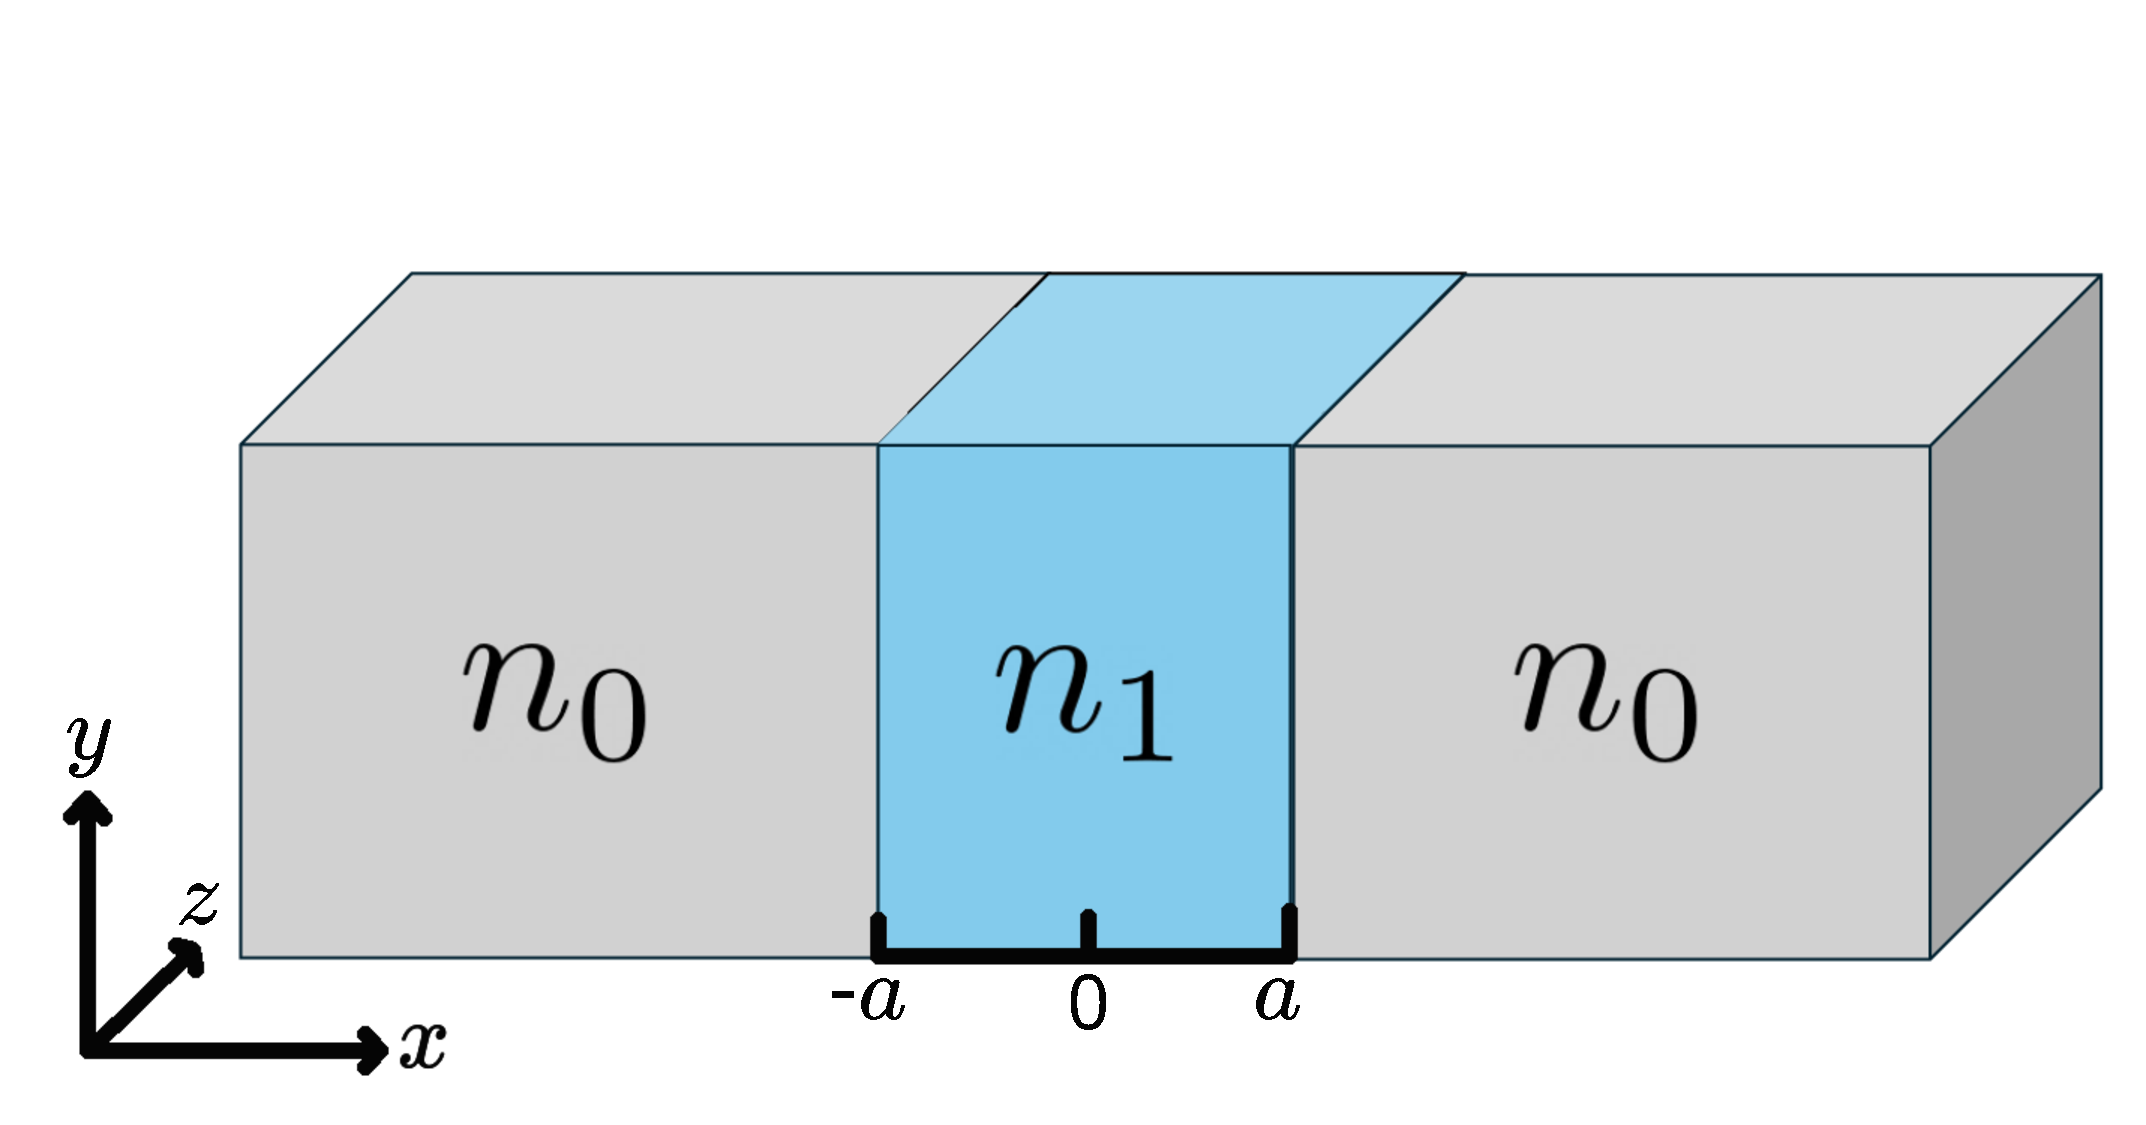
\includegraphics[width=0.6\linewidth]{media/slab.pdf}
	\caption[Forma de una guía de onda tipo losa.]{Forma de una guía de onda tipo losa. En las direcciones $\mathbf{\hat{y}}$ (vertical) y $\mathbf{\hat{z}}$ (hacia dentro de la página) la estructura es invariante.}
\end{figure}

Dado que $\nabla n^2 = \textbf{0}$ para $|x| \neq a$, los lados derechos de las ecuaciones (\ref{eqn:helmholz}) y (\ref{eqn:helmholzH}) son de tipo Helmholz. Definiendo $\Psi = \{E_z, H_z\} $:
\begin{align*}
	(\nabla_\perp^2  + k_0^2n^2 - k_z^2) \Psi  &=  \frac{d^2\Psi}{dx^2} + (k_0^2n^2 - k_z^2) \Psi  = 0.
\end{align*}
Dado que $n(x)=n(-x)$, las soluciones $\Psi$ deben ser pares o impares. Para encontrar soluciones cuya energía esté localizada en la guía de onda y que decaiga fuera de ella, se impondrá $k_0^2n_0^2 \le k_z^2 \le k_0^2n_1^2$. Se hace natural definir $\alpha^2\equiv k_0^2n_1^2-k_z^2$ y $\beta^2\equiv k_z^2 - k_0^2n_0^2$. Con todo ésto, 
\begin{equation*}
	\Psi_s = \left\{\begin{matrix}
	\Psi_{s1}\cos(\alpha x),\quad |x|\le a
	\\
	\Psi_{s0}e^{-\beta|x|}, \quad |x|>a
	\end{matrix}\right.
\end{equation*}

\begin{equation*}
	\nabla_\perp \Psi_s = \left\{\begin{matrix}
	-\hat{\textbf{x}}\alpha\Psi_{s1}\sin(\alpha x),\quad |x|\le a
	\\
	-\hat{\textbf{x}}\frac{|x|}{x}\beta\Psi_{s0}e^{-\beta|x|}, \quad |x|>a
	\end{matrix}\right.
\end{equation*}
Por lo que las componentes verticales $E_y$ y $H_y$ pares se escriben debido a la ecuación (\ref{eqn:transversal}) como:
\begin{equation*}
	\begin{aligned}[c]
	 E_y &= \frac{i}{k_0^2n^2-k_z^2} \left\{\begin{matrix}
	 \omega\mu_0\alpha H_{s1}\sin(\alpha x),	 \quad |x|\le a
	 \\
	 \omega\mu_0\frac{|x|}{x}\beta H_{s0}e^{-\beta|x|},\quad |x|>a
	 \end{matrix}\right.
\end{aligned} 
\quad
	\begin{aligned}[c]
	 H_y &= \frac{i}{k_0^2n^2-k_z^2} \left\{\begin{matrix}
	 -\omega \epsilon_0 n^2\alpha E_{s1}\sin(\alpha x),	 \quad |x|\le a
	 \\
	 -\omega \epsilon_0 n^2\frac{|x|}{x}\beta E_{s0}e^{-\beta|x|},\quad |x|>a
	 \end{matrix}\right.
\end{aligned} 
\end{equation*}
Por otro lado, las soluciones impares tienen la forma
\begin{equation*}
	\Psi_a = \left\{\begin{matrix}
	\Psi_{a1}\sin(\alpha x),\quad |x|\le a
	\\
	\Psi_{a0}e^{-\beta|x|}, \quad |x|>a
	\end{matrix}\right.
\end{equation*}
\begin{equation*}
	\nabla_\perp \Psi_a = \left\{\begin{matrix}
	\hat{\textbf{x}}\alpha\Psi_{a1}\cos(\alpha x),\quad |x|\le a
	\\
	-\hat{\textbf{x}}\frac{|x|}{x}\beta\Psi_{a0}e^{-\beta|x|}, \quad |x|>a
	\end{matrix}\right.
\end{equation*}
Por lo que $E_y$ y $H_y$ se escriben como:
\begin{equation*}
	\begin{aligned}[c]
	 E_y &= \frac{i}{k_0^2n^2-k_z^2} \left\{\begin{matrix}
	 -\omega\mu_0\alpha H_{a1}\cos(\alpha x)	, \quad |x|\le a
	 \\
	 \omega\mu_0\frac{|x|}{x}\beta H_{a0}e^{-\beta|x|},\quad |x|>a
	 \end{matrix}\right.
\end{aligned} 
\quad
	\begin{aligned}[c]
	 H_y &= \frac{i}{k_0^2n^2-k_z^2} \left\{\begin{matrix}
	 \omega \epsilon_0 n^2 \alpha E_{a1}\cos(\alpha x),	 \quad |x|\le a
	 \\
	 -\omega \epsilon_0 n^2 \frac{|x|}{x}\beta E_{a0}e^{-\beta|x|},\quad |x|>a
	 \end{matrix}\right.
\end{aligned} .
\end{equation*}
Imponiendo continuidad de $E_y$, $E_z$, $H_y$ y $H_z$, tratando los casos par e impar por separado:
\begin{equation*}
	\begin{aligned}[c]
	 E_{s1}\cos(\alpha a) = E_{s0}e^{-\beta a},
	 \\	 
	 H_{s1}\cos(\alpha a) = H_{s0}e^{-\beta a},
	 \\
	 	  n_1 ^2 E_{s1}\sin(\alpha a)/\alpha = -n_0^2 E_{s0}e^{-\beta a}/\beta,
	  \\
	  H_{s1}\sin(\alpha a)/\alpha = - H_{s0}e^{-\beta a}/\beta,
\end{aligned} 
\quad
	\begin{aligned}[c]
		 E_{a1}\sin(\alpha a) = E_{a0}e^{-\beta a},
	 	   \\
	 H_{a1}\sin(\alpha a) = H_{a0}e^{-\beta a},
	 \\
	  n_1 ^2 E_{a1}\cos(\alpha a)/\alpha = n_0^2 E_{a0}e^{-\beta a}/\beta,
	 	 \\
	  H_{a1}\cos(\alpha a)/\alpha = H_{a0}e^{-\beta a}/\beta.
\end{aligned} 
\end{equation*}
Buscando soluciones no triviales se tiene que:
\begin{equation*}
	\begin{aligned}[c]
	\left[\frac{\cos(\alpha a)}{\beta a} + \frac{\sin(\alpha a)}{\alpha a}\right] \left[n_0^2 \frac{\cos(\alpha a)}{\beta a} + n_1^2\frac{\sin(\alpha a)}{\alpha a} \right] = 0,
\end{aligned} 
\quad
	\begin{aligned}[c]
	 \left[ \frac{\sin(\alpha a)}{\beta a} - \frac{\cos(\alpha a)}{\alpha a}\right]\left[ n_0^2\frac{\sin(\alpha a)}{\beta a} - n_1^2\frac{\cos(\alpha a)}{\alpha a}\right] = 0
\end{aligned} .
\end{equation*}
Se distinguirá dos tipos de condiciones:
\begin{align*}
	\frac{\cos(\alpha a)}{\beta a} + \frac{\sin(\alpha a)}{\alpha a}&= 0, & n_0^2 \frac{\cos(\alpha a)}{\beta a} + n_1^2\frac{\sin(\alpha a)}{\alpha a}  &= 0,
	\\
	&\qquad\text{(modos TE)}	& &\qquad\text{(modos TM)}	
	\\
	 \frac{\sin(\alpha a)}{\beta a} - \frac{\cos(\alpha a)}{\alpha a} &= 0, &  n_0^2\frac{\sin(\alpha a)}{\beta a} - n_1^2\frac{\cos(\alpha a)}{\alpha a} &= 0.
\end{align*}
Asumiendo $\alpha$, $\beta$ y $k_z$ conocidos, las amplitudes deben cumplir las relaciones:
\begin{equation*}
	\begin{aligned}[c]
	E_{s1} \left[n_0^2 \frac{\cos(\alpha a)}{\beta a}+n_1 ^2 \frac{\sin(\alpha a)}{\alpha a}\right] = 0,
		\\
	H_{s1} \left[\frac{\cos(\alpha a)}{\beta a} + \frac{\sin(\alpha a)}{\alpha a} \right] = 0,
\end{aligned} 
\quad\quad
	\begin{aligned}[c]
	E_{a1} \left[ n_0^2\frac{\sin(\alpha a)}{\beta a} - n_1^2\frac{\cos(\alpha a)}{\alpha a}\right] = 0,
		\\
	H_{a1} \left[ \frac{\sin(\alpha a)}{\beta a} - \frac{\cos(\alpha a)}{\alpha a}\right] = 0.
\end{aligned} 
\end{equation*}
Las ecuaciones superiores imponen que $E_1 = 0$ cuando se satisface la condición de modos TE. Análogamente, las ecuaciones inferiores imponen $H_1 = 0$ en el caso de modos TM. Efectivamente, los nombres TE y TM se han puesto por transversal eléctrico y transversal magnético, respectivamente.
Un corolario para los modos TE es que $E_z = E_x = 0$ por lo que la polarización del campo eléctrico será exclusivamente en la dirección $\hat{\textbf{y}}$. Sólo un haz polarizado en $\hat{\textbf{x}}$ podría excitar un modo TM, por lo que en un experimento se debe tener esto presente.

\subsection{Modos TE}

Usando las dos ecuaciones de modos TE junto a la restricción $(\alpha a)^2 + (\beta a)^2 = k_0^2 a^2(n_1^2 - n_0^2) \equiv V^2$ es posible obtener soluciones gráficas para las constantes de propagación $k_z$.

\begin{figure}[H]
	\centering
	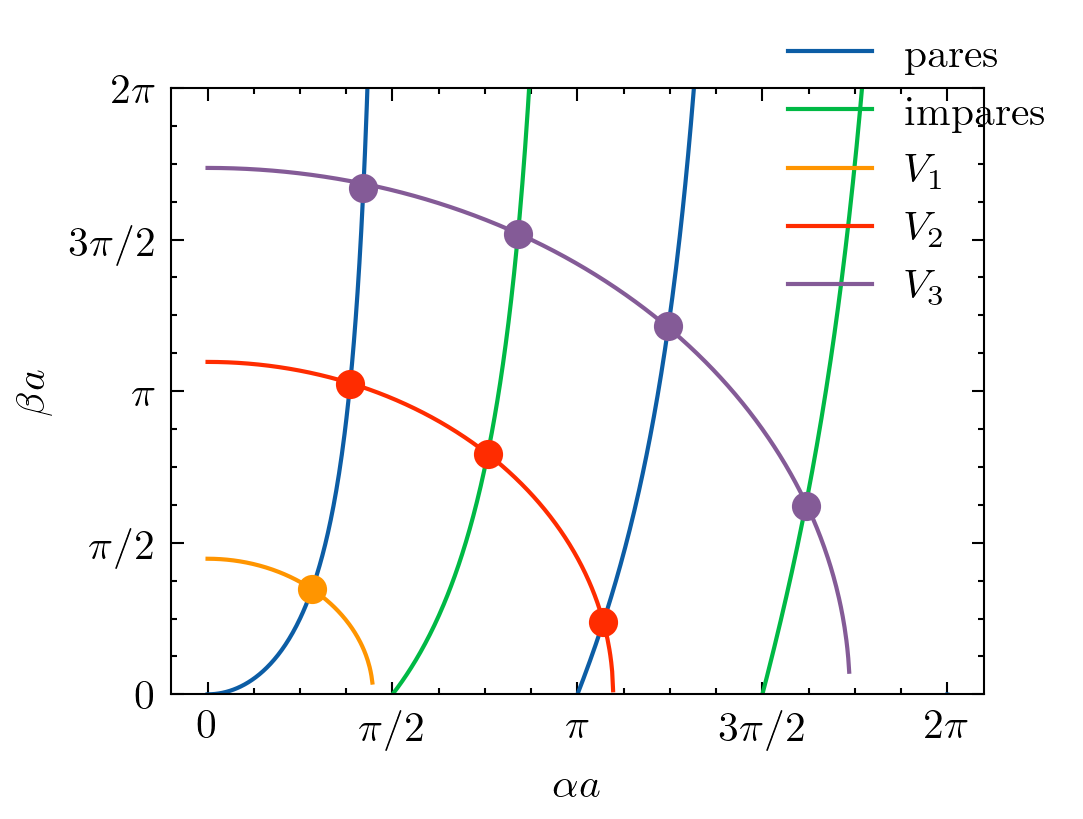
\includegraphics[width=0.7\linewidth]{media/slabgraphical}
	\caption[Soluciones gráficas de los modos TE]{Soluciones gráficas de los modos TE. A mayor contraste $\Delta n = n_1-n_0$, mayor cantidad de modos guiados soporta la guía de onda.}
\end{figure}
\subsection{Modos TM}

\begin{figure}[H]
	\centering
	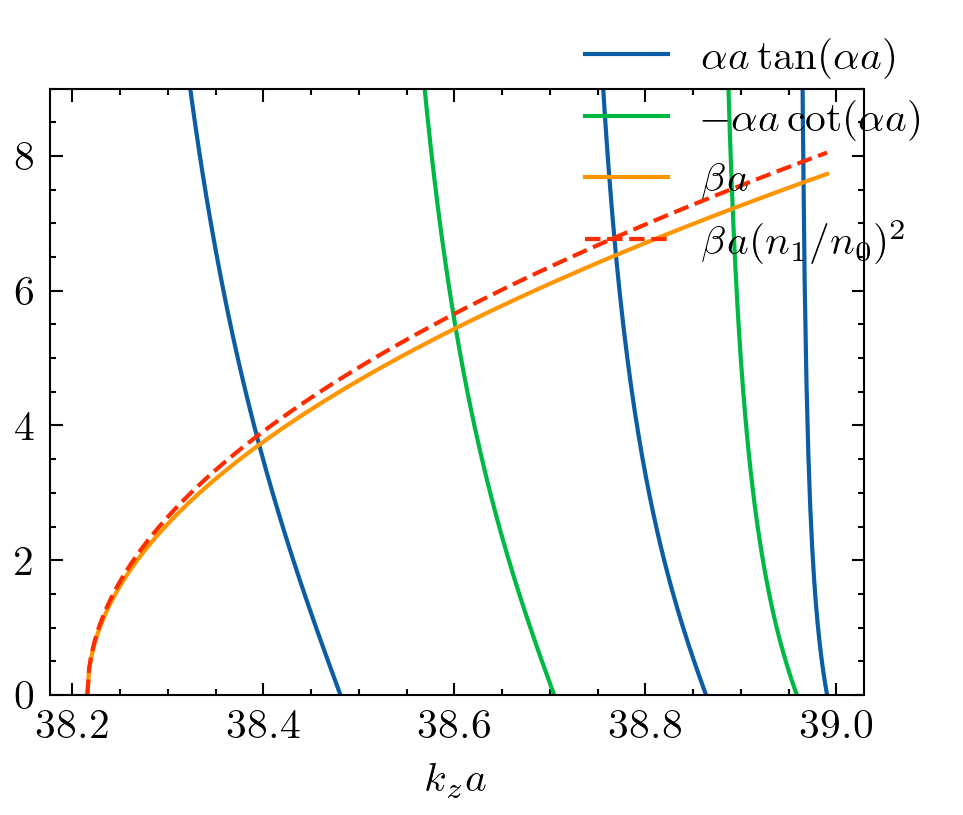
\includegraphics[width=0.6\linewidth]{media/slabgraphicalTETM1}
	\caption[Soluciones gráficas de los modos TE y TM]{Soluciones gráficas de los modos TE y TM para $\Delta n = 3\times 10^{-2}$. Se aprecia que las constantes de propagación de los modos TM (rojo discontinuo) son menores que las de los modos TE (naranjo liso).}
\end{figure}
\section{Soluciones analíticas para fibra óptica circular}
En la sección anterior se estudió el sistema más sencillo en el que se puede hablar de guías de onda dieléctricas. El siguiente paso en complejidad consiste en guías de onda circulares. Para ello, se considerará que el índice de refracción varía radialmente según 
\begin{equation}
	n( \rho ) = 
	\left\{\begin{matrix}
	n_1, \quad \text{si } \rho \le a
	\\
	n_0, \quad \text{si } \rho > a
	\end{matrix}\right.
	,\nonumber
\end{equation}
donde la tupla $(\rho, \phi, z)$ define las coordenadas cilíndricas a usar, más apropiadas para este problema. Al considerar las componentes longitudinales $\Psi$ = $\{E_z, H_z\}$ del campo eléctrico y magnético, respectivamente, usando separación de variables $\Psi =  R(\rho)\Phi(\phi) e^{ik_z z} $ las ecuaciones (\ref{eqn:helmholz}) y (\ref{eqn:helmholzH}) toman la forma:

\begin{align}
	\left[\frac{\partial^2}{\partial \rho^2} + \frac{\partial}{\rho\partial \rho} + \frac{\partial^2}{\rho^2\partial \phi^2} +\left( k_0^2n^2 - k_z^2 \right)\right]  R(\rho)\Phi(\phi) = 0
	\nonumber
	\\
\rho^2\frac{d^2 R}{Rd\rho^2} + \rho\frac{dR}{Rd\rho} + \rho^2\left( k_0^2n^2 - k_z^2 \right) + \underbrace{\frac{d^2 \Phi}{\Phi d\phi^2}}_{-\ell^2} = 0
\nonumber
\\
\therefore \Phi(\phi) = A e^{i\ell\phi}
\nonumber
\end{align}
Imponiendo condiciones de periodicidad $\Phi(\phi)=\Phi(\phi + 2\pi)$, se tiene necesariamente que $\ell$ es un número entero. Por consiguiente, la ecuación para $R(\rho)$ es de tipo Bessel entera, por lo que buscando soluciones tales que $k_0^2 n_0^2 < \beta_z^2 < k_0^2 n_1^2$ y definiendo nuevamente $\alpha^2 \equiv k_0^2n_1^2 - k_z^2$ y $\beta^2\equiv k_z^2 - k_0^2n_0^2$ se tiene:
\begin{align}
	\frac{d^2 R}{d\rho^2} + \frac{1}{\rho}\frac{dR}{d\rho} + \left( k_0^2n^2 - k_z^2 -\frac{\ell^2}{\rho^2}\right)R  = 0
	\nonumber
	\\
	\therefore R(\rho) = 
	\left\{
	\begin{matrix}	
	C_1 J_\ell (\alpha\rho) + D_1 Y_\ell (\alpha\rho), \quad \text{si } \rho \le a  
	\\
	C_2 K_\ell (\beta\rho) + D_2 I_\ell (\beta\rho), \quad \text{si } \rho > a  
	\end{matrix}
	\right.
	. \nonumber
\end{align}
Necesariamente se debe imponer $D_1 = D_2 = 0$ para que la solución sea finita para $\rho = 0$ y para $\rho \to +\infty$. Es decir, la parte radial de la solución es
\begin{align*}
 R(\rho) = 
	\left\{
	\begin{matrix}	
	C_1 J_\ell (\alpha\rho), \quad \text{si } \rho \le a  
	\\
	C_2 K_\ell (\beta\rho), \quad \text{si } \rho > a  
	\end{matrix}
	\right.
	. \nonumber
\end{align*}
En este caso, para imponer las condiciones de continuidad en $\textbf{E}_{||} = E_\phi \boldsymbol{\hat{\phi}} + E_z \hat{\textbf{z}}$ y $\textbf{H}_{||}= H_\phi \hat{\boldsymbol{\phi}} + H_z \hat{\textbf{z}}$, se hace necesario relacionar el resto de componentes del campo con $E_z$ y $H_z$ para lo cual se usará la ecuación (\ref{eqn:transversal}). 

Como 
\begin{equation*}
	\nabla_\perp \Psi =
	\left\{	
	\begin{matrix}
		\Psi_0^1\left[\boldsymbol{\hat{\rho}}\alpha J'_\ell (\alpha \rho) + i \boldsymbol{\hat{\phi}} \ell J_\ell (\alpha \rho)/\rho\right] e^{i\ell\phi} e^{i k_z z}, \quad \text{si } \rho \le a  
		\\
		\Psi_0^0\left[\boldsymbol{\hat{\rho}}\beta K'_\ell (\beta\rho) +i \boldsymbol{\hat{\phi}}\ell K_\ell (\alpha \rho)/\rho \right]e^{i\ell\phi} e^{i k_z z} , \quad \text{si } \rho > a  
	\end{matrix}
	\right.
\end{equation*}

Separando por componentes y reemplazando:
\begin{align*}
		H_z &=  e^{i\ell\phi}e^{i k_z z}
	  	 \left\{
		\begin{matrix}	  	 
	  	 H_0^1 J_\ell (\alpha \rho), \quad \text{si } \rho \le a  
	  	 \\
	  	 H_0^0 K_\ell (\beta \rho), \quad \text{si } \rho > a  
	  	 \end{matrix}
	  	 \right.	
		\\
	  	 H_r &= \frac{i e^{i\ell\phi}e^{i k_z z} }{k_0^2 n^2 - k_z^2}
	  	 \left\{
		\begin{matrix}	  	 
	  	  k_z \alpha H_0^1 J'_\ell (\alpha \rho) - i\omega \epsilon_0 n^2\ell E_0^1 J_\ell (\alpha \rho)/\rho, \quad \text{si } \rho \le a  
	  	 \\
	  	 k_z \beta H_0^0  K'_\ell (\beta \rho) - i\omega \epsilon_0 n^2\ell E_0^0 K_\ell (\beta \rho)/\rho  , \quad \text{si } \rho > a  
	  	 \end{matrix}
	  	 \right.
	  	 \\
		H_\phi &= \frac{ie^{i\ell\phi} e^{i k_z z}}{k_0^2 n^2 - k_z^2}
		\left\{
		\begin{matrix}
			\omega \epsilon_0 n^2  \alpha E_0^1 J'_\ell (\alpha \rho)+ik_z\ell H_0^1  J_\ell (\alpha \rho)/\rho, \quad \text{si } \rho \le a  
			\\
			\omega \epsilon_0 n^2 \beta E_0^0  K'_\ell (\beta \rho)+ik_z \ell H_0^0  K_\ell (\beta \rho)/\rho , \quad \text{si } \rho > a  
		\end{matrix}
		\right.
		\\
		E_z &= e^{i\ell\phi} e^{i k_z z}
	  	 \left\{
		\begin{matrix}	  	 
	  	 E_0^1 J_\ell (\alpha \rho), \quad \text{si } \rho \le a  
	  	 \\
	  	 E_0^0 K_\ell (\beta \rho), \quad \text{si } \rho > a  
	  	 \end{matrix}
	  	 \right.	
		\\
	E_r &= \frac{i e^{i\ell\phi} e^{i k_z z} }{k_0^2 n^2 - k_z^2}
	  	 \left\{
		\begin{matrix}	  	 
	  	  k_z \alpha E_0^1 J'_\ell (\alpha \rho)+i\omega \mu_0 \ell H_0^1 J_\ell (\alpha \rho)/\rho , \quad \text{si } \rho \le a  
	  	 \\
	  	 k_z \beta E_0^0  K'_\ell (\beta \rho) +i\omega \mu_0 \ell H_0^0 K_\ell (\beta \rho)/\rho, \quad \text{si } \rho > a  
	  	 \end{matrix}
	  	 \right.
	\\
	E_\phi &= \frac{i e^{i\ell\phi} e^{i k_z z}}{k_0^2 n^2 - k_z^2}
		\left\{
		\begin{matrix}
			ik_z \ell E_0^1   J_\ell (\alpha \rho)/\rho -\omega \mu_0  \alpha H_0^1  J'_\ell (\alpha \rho), \quad \text{si } \rho \le a  
			\\
			ik_z \ell E_0^0   K_\ell (\beta \rho)/\rho -\omega \mu_0 \beta H_0^0   K'_\ell (\beta \rho) , \quad \text{si } \rho > a  
		\end{matrix}
		\right.
\end{align*}

Ahora sí, imponiendo continuidad:
\begin{align}
	H_0^{1} J_\ell(\alpha a) &= H_0^{0} K_\ell (\beta a)
	\label{eqn:cont1}
	\\
	E_0^{1} J_\ell(\alpha a) &= E_0^{0} K_\ell (\beta a)
	\label{eqn:cont2}
	 \\
	 -\omega \epsilon_0 n_1^2  \alpha\beta^2 a E_0^1 J'_\ell (\alpha a)-ik_z\ell \beta^2 H_0^1  J_\ell (\alpha a)
	 &= \omega \epsilon_0 n_0^2 \alpha^2 \beta a E_0^0 K'_\ell (\beta a)+ik_z\ell \alpha^2H_0^0  K_\ell (\beta a)
	 \label{eqn:cont3}
	 \\
	 -ik_z \ell \beta^2 E_0^1   J_\ell (\alpha a) + \omega \mu_0  \alpha \beta^2 a H_0^1  J'_\ell (\alpha a) &=
	 ik_z \ell \alpha^2 E_0^0   K_\ell (\beta a) -\omega \mu_0  \alpha^2 \beta a H_0^0  K'_\ell (\beta a)
	 \label{eqn:cont4}
\end{align}
Buscando soluciones no triviales:
\begin{align*}
	\left|\begin{matrix}
		K_\ell(\beta a) & -J_\ell(\alpha a) & 0 & 0
		\\
		0 & 0 & K_\ell(\beta a) & -J_\ell(\alpha a)
		\\
		ik_z\ell \alpha^2 K_\ell (\beta a) & ik_z\ell\beta^2 J_\ell (\alpha a) & \omega \epsilon_0 n_0^2  \alpha^2 \beta a K'_\ell (\beta a) & \omega \epsilon_0 n_1^2  \alpha \beta^2 a J'_\ell (\alpha a)
		\\
		\omega \mu_0  \alpha^2 \beta a   K'_\ell (\beta a) &  \omega \mu_0  \alpha \beta^2 a J'_\ell (\alpha a) & -ik_z \ell \alpha^2 K_\ell (\beta a) &  -ik_z \ell \beta^2  J_\ell (\alpha a)
	\end{matrix}\right|
	=
0
\end{align*}
Finalmente, la ecuación trascendental que satifacen $\alpha$, $\beta$ y $k_z$ es:
\begin{equation}
	\left( \frac{J_\ell'(\alpha a)}{\alpha a J_\ell(\alpha a)} + \frac{K_\ell'(\beta a)}{\beta a K_\ell(\beta a)} \right)\left( n_1^2\frac{J_\ell'(\alpha a)}{\alpha a J_\ell(\alpha a)} + n_0^2\frac{K_\ell'(\beta a)}{\beta a K_\ell(\beta a)} \right) = \ell^2 \left[ \left(\frac{1}{\alpha a}\right)^2 + \left(\frac{1}{\beta a}\right)^2 \right]^2 \left( \frac{k_z}{k_0} \right)^2 \label{eqn:fiber_trascendental}
\end{equation}

Dado que, en principio, los valores de $k_z$ ya están determinados por la ecuación anterior, es posible obtener dos relaciones entre $H_0^1$ y $E_0^1$:
\begin{align}
\frac{E_0^1}{H_0^1} &=  -\frac{i k_z \ell}{\omega\epsilon_0}\left[ \left(\frac{1}{\alpha a}\right)^2 + \left(\frac{1}{\beta a}\right)^2 \right]  \left[ n_1^2 \frac{J'_\ell(\alpha a)}{\alpha a J_\ell(\alpha a)} + n_0^2 \frac{K'_\ell(\beta a)}{\beta a K_\ell(\beta a)} \right]^{-1} \label{eqn:fiber_polarization_E}
\\
\frac{H_0^1}{E_0^1} &=  \frac{i k_z \ell}{ \omega\mu_0}\left[ \left(\frac{1}{\alpha a}\right)^2 + \left(\frac{1}{\beta a}\right)^2 \right]  \left[ \frac{J'_\ell(\alpha a)}{\alpha a J_\ell(\alpha a)} + \frac{K'_\ell(\beta a)}{\beta a K_\ell(\beta a)} \right]^{-1} \label{eqn:fiber_polarization_H}
\end{align}

\subsection{Modos TE y TM}
El caso más sencillo de estudiar es imponiendo $\ell = 0$. La ecuación (\ref{eqn:fiber_trascendental}) implica:
\begin{align*}
	\frac{J'_{0}(\alpha a)}{\alpha a J_0(\alpha a)} + \frac{K'_0(\beta a)}{\beta a K_0(\beta a)}&=  0, \quad \text{(modos TE)}
	\\
	n_1^2\frac{J'_{0}(\alpha a)}{\alpha a J_0(\alpha a)} + n_0^2 \frac{K'_0(\beta a)}{\beta a K_0(\beta a)} &= 0, \quad \text{(modos TM)}
\end{align*}

De las ecuaciones (\ref{eqn:fiber_polarization_E}) y (\ref{eqn:fiber_polarization_H}) es directo notar que la condiciones de modos transversales impiden que el denominador se anule, lo que permite afirmar sin ambigüedad que las componentes longitudinales se hacen cero para $\ell = 0$ en los casos respectivos: $H_0^1 = 0$ para TE y $E_0^1 = 0$ para TM.


\subsection{Modos HE y EH}
Interpretando la ecuación (\ref{eqn:fiber_trascendental}) como una cuadrática en $J_\ell'(\alpha a)/\alpha a J_\ell(\alpha a)$:
\begin{align*}
	\frac{J_\ell'(\alpha a)}{\alpha a J_\ell(\alpha a)} &= -\left(\frac{n_1^2+n_0^2}{2n_1^2}\right) \frac{K_\ell'(\beta a)}{\beta a K_\ell(\beta a)}\pm\sqrt{\left(\frac{n_1^2-n_0^2}{2n_1^2}\right)^2\left(\frac{K_\ell'(\beta a)}{\beta a K_\ell(\beta a)}\right)^2+ \left( \frac{ k_z \ell}{ k_0 n_1} \right)^2\left[ \left(\frac{1}{\alpha a}\right)^2 + \left(\frac{1}{\beta a}\right)^2 \right]^2 }
\end{align*}

Haciendo uso de las relaciones de recurrencia de las funciones de Bessel $J_\ell(r)$,  es posible obtener dos tipos de soluciones llamadas HE y EH:

\begin{align}
		\frac{J_{\ell-1}(\alpha a)}{\alpha a J_\ell(\alpha a)} &= -\left(\frac{n_1^2+n_0^2}{2n_1^2}\right) \frac{K_\ell'(\beta a)}{\beta a K_\ell(\beta a)}+\frac{\ell}{(\alpha a)^2}-\sqrt{\Delta}, \quad \text{(modos HE)}
		\label{eqn:HE}
	\\
		\frac{J_{\ell+1}(\alpha a)}{\alpha a J_\ell(\alpha a)} &= \left(\frac{n_1^2+n_0^2}{2n_1^2}\right) \frac{K_\ell'(\beta a)}{\beta a K_\ell(\beta a)}+\frac{\ell}{(\alpha a)^2}-\sqrt{\Delta}, \quad \text{(modos EH)}
		\label{eqn:EH}
		\\
		\Delta &= \left(\frac{n_1^2-n_0^2}{2n_1^2}\right)^2\left(\frac{K_\ell'(\beta a)}{\beta a K_\ell(\beta a)}\right)^2+ \left( \frac{ k_z \ell}{ k_0 n_1} \right)^2\left[ \left(\frac{1}{\alpha a}\right)^2 + \left(\frac{1}{\beta a}\right)^2 \right]^2 \nonumber
\end{align}



\section{Modos normales en guías de onda}

Si la estructura de guías de onda no varía en la dirección $z$, el campo eléctrico se puede expresar como una onda plana del tipo $\textbf{E}(\textbf{r}) = \textbf{E}_\nu(x, y) e^{i\beta_\nu z}$. A su vez, es conveniente separar el Laplaciano como $\nabla^2 \equiv \nabla_\perp^2 + \frac{\partial^2}{\partial z^2}$. De esta forma, el lado izquierdo de las ecuaciones (\ref{eqn:helmholz}), se desarrolla como:

\begin{align}
	(\nabla^2  + k_0^2n^2) \textbf{E}(\textbf{r}) &= \left(\nabla_\perp^2 + \frac{\partial^2}{\partial z^2} + k_0^2n^2\right) \textbf{E}_\nu(x, y)  e^{i\beta_\nu z} \nonumber
\\	
	&= e^{i\beta_\nu z} \nabla_\perp^2 \textbf{E}_\nu -\beta_\nu^2\textbf{E}_\nu e^{i\beta_\nu z} + k_0^2n^2 \textbf{E}_\nu  e^{i\beta_\nu z}
\nonumber	
	\\	
	&= \left[  \nabla_\perp^2  + (k_0^2n^2-\beta_\nu^2) \right]\textbf{E}_\nu  e^{i\beta_\nu z}
	\nonumber	
	\\
	&\approx
	0
	\nonumber
	\\
	\therefore
	 \left[  \nabla_\perp^2  + k_0^2n^2(x,y) \right]&\textbf{E}_\nu(x,y)  = \beta_\nu^2 \textbf{E}_\nu(x,y), \label{eqn:eigenfield}
\end{align}
donde se ha usado la aproximación de guiaje débil para anular el lado de derecho de la ecuación (\ref{eqn:helmholz}). Notemos que la ecuación (\ref{eqn:eigenfield}) es un problema de autovalores $\beta_\nu^2$ y autofunciones $\textbf{E}_\nu(x,y)$, que son ortogonales y forman una base completa (ver apéndice \ref{sec:orto}). En principio, la forma espacial del índice de refracción $n(x, y)$ puede ser arbitraria siempre y cuando que se satisfaga la condición de guiaje débil. 

\section{Teoría de modos acoplados}
	Para el estudio de redes fotónicas, es conveniente utilizar herramientas similares a las de la Física del Sólido en lo que respecta a potenciales periódicos. En particular, se puede suponer que los modos guiados de una guía de onda están fuertemente ligados a ella (enlace fuerte o \textit{Tight Binding}), incluso en presencia de otras guías de onda. Es decir, se supondrá que el $\nu$-ésimo modo de la $m$-ésima guía de onda satisface para toda distancia de propagación $z$ la ecuación (\ref{eqn:eigenfield}), donde el índice de refracción total se puede descomponer en una suma periódica de guías de onda $n^2(\textbf{r}) = \sum_{m} n^2_m(\textbf{r})$. Entonces, descomponiendo el campo eléctrico total de la forma $\textbf{E}(\textbf{r}) = \sum_{\nu, m} \textbf{E}_{\nu, m}(x, y) a_{\nu, m}(z) e^{i\beta_{\nu, m} z}$ y reemplazando en la ecuación (\ref{eqn:helmholz}) se tiene:

\begin{align}
	(\nabla^2  + k_0^2n^2) \textbf{E}(\textbf{r}) &= \left(\nabla_\perp^2 + \frac{\partial^2}{\partial z^2} + k_0^2n^2 \right)\sum_{\nu, m} \textbf{E}_{\nu, m}(x, y) a_{\nu, m}(z) e^{i\beta_{\nu, m} z}
	\nonumber
	\\
	&= \sum_{\nu, m} \left[a_{\nu, m} e^{i\beta_{\nu, m} z} \left(\nabla_\perp^2 +k_0^2n^2 \right)\textbf{E}_{\nu, m} + \textbf{E}_{\nu, m}\frac{d^2}{d z^2}\left(a_{\nu, m} e^{i\beta_{\nu, m} z}\right)\right]
	\nonumber	
	\\
	&= \sum_{\nu, m} \left[a_{\nu, m}  \left(\nabla_\perp^2 +k_0^2n^2 -\beta_{\nu,m}^2 \right) + \frac{d^2 a_{\nu, m}}{d z^2}  +2i\beta_{\nu,m}\frac{d a_{\nu, m}}{d z} \right]e^{i\beta_{\nu, m} z}\textbf{E}_{\nu, m}
		\nonumber	
	\\
	&\approx \sum_{\nu, m} \left[a_{\nu, m}  k_0^2(n^2 - n^2_{m}) +2i\beta_{\nu,m}\frac{d a_{\nu, m}}{d z} \right]e^{i\beta_{\nu, m} z}\textbf{E}_{\nu, m}
	\nonumber	
	\\
	&= 0,
	\nonumber	
\end{align}
donde se ha usado que $\left|\frac{d^2 a_{\nu, m}}{d z^2}\right|\ll 2\beta_{\nu,m}\left|\frac{d a_{\nu, m}}{d z}\right|  $, conocida como aproximación paraxial. Aplicando producto punto con $\textbf{E}_{\mu, m'}^*$ e integrando en todo el plano $xy$:
\begin{align}
	  \int\displaylimits_{-\infty}^{+\infty}\int\displaylimits_{-\infty}^{+\infty} \sum_{\nu, m} \left[a_{\nu, m}  k_0^2(n^2 - n^2_{m}) +2i\beta_{\nu,m}\frac{d a_{\nu, m}}{d z} \right]e^{i\beta_{\nu, m} z}\textbf{E}_{\nu, m} \cdot \textbf{E}_{\mu, m'}^* dxdy &= 0
	  \nonumber
	  \\
	  \sum_{\nu, m} \left(2i\beta_{\nu,m}\frac{d a_{\nu, m}}{d z} \delta_{\nu,\mu}\delta_{m,m'} +  2\beta_{\mu, m'}C_{m', m, \nu, \mu}   a_{\nu, m} \right)e^{i\beta_{\nu, m} z} &= 0
	  \nonumber
	  \\
	  	  i\frac{d a_{\mu, m'}}{d z} e^{i\beta_{\mu, m'} z} +  \sum_{\nu, m\neq m'}C_{m', m, \nu, \mu}   a_{\nu, m} e^{i\beta_{\nu, m} z} &= 0,
	  	  \nonumber
\end{align}
donde se han definido y usado
\begin{align*}
	   C_{m', m, \nu, \mu} &\equiv \frac{k_0^2}{2\beta_{\mu, m'}}\int\displaylimits_{-\infty}^{+\infty}\int\displaylimits_{-\infty}^{+\infty} (n^2 - n^2_{m}) \textbf{E}_{\nu, m} \cdot \textbf{E}_{\mu, m'}^* dxdy , \quad\int\displaylimits_{-\infty}^{+\infty}\int\displaylimits_{-\infty}^{+\infty} \textbf{E}_{\nu, m} \cdot \textbf{E}_{\mu, m'}^* dxdy \approx \delta_{\nu,\mu}\delta_{m,m'}.
\end{align*}

Es decir, el efecto del modo $(\nu, m)$ en la dinámica del modo $(\mu, m')$ sólo es apreciable al ponderar con la expresión $(n^2 - n^2_{m})$, lo que da origen al término $C_{m', m, \nu, \mu}$ conocido comúnmente como constante de acoplamiento. Sin el peso del contraste, la interacción es evanescente, por lo que la aproximación de ortogonalidad se hace razonable con suficiente distancia entre guías (sobre los 15 $\mu$m en los experimentos de esta tesis). Cuando $m=m'$, el acoplamiento $C_{m', m, \nu, \mu}$ es nulo por definición.

Finalmente, es posible hacer el cambio de variables $u_{\nu, m} \equiv a_{\nu, m} e^{i\beta_{\nu, m} z}$ para llegar a las llamadas ecuaciones discretas tipo Schrödinger:
\begin{equation}
	  	 -i\frac{d u_{\mu, m'}}{dz} = \beta_{\mu, m'} u_{\mu, m'} + \sum_{\nu, m\neq m'}C_{m', m, \nu, \mu}   u_{\nu, m}.
	\label{eqn:CMT1}
\end{equation}



Para fijar ideas, consideremos el caso del dímero monomodal homogéneo, considerando una distancia $d$ entre guías \textcolor{red}{INCLUIR ESQUEMA PARA EXPLICAR ACOPLAMIENTO}. El índice de refracción en este caso es $n^2 = n_1^2 + n_2^2$, con $n_1^2(\textbf{r})=n_2^2(\textbf{r}+\textbf{d})$. Dada la simetría del problema, la constante de acoplamiento se puede desarrollar como 
\begin{align}
	C_{1, 2} &=  \frac{1}{2\beta}\int\displaylimits_{-\infty}^{+\infty}\int\displaylimits_{-\infty}^{+\infty} k_0^2 n_1^2(\textbf{r}) \textbf{E}_{2}(\textbf{r}) \cdot \textbf{E}_{1}^*(\textbf{r}) dxdy 
	= \frac{k_0^2}{2\beta}\int\displaylimits_{-\infty}^{+\infty}\int\displaylimits_{-\infty}^{+\infty}  n_2^2(\textbf{r}+\textbf{d}) \textbf{E}_{1}(\textbf{r}+\textbf{d}) \cdot \textbf{E}_{1}^*(\textbf{r}) dxdy 
	\nonumber	
	\\	
	&= \frac{k_0^2}{2\beta}\int\displaylimits_{-\infty}^{+\infty}\int\displaylimits_{-\infty}^{+\infty} n_2^2(\textbf{r}) \textbf{E}_{1}(\textbf{r}) \cdot \textbf{E}_{1}^*(\textbf{r}-\textbf{d}) dxdy 
	= \frac{k_0^2}{2\beta}\int\displaylimits_{-\infty}^{+\infty}\int\displaylimits_{-\infty}^{+\infty} n_2^2(\textbf{r}) \textbf{E}_{1}(\textbf{r}) \cdot \textbf{E}_{2}^*(\textbf{r}) dxdy 
	\nonumber
	\\	
	&= C_{2,1} \equiv C
	\nonumber
\end{align}
 por lo que las dos ecuaciones dinámicas se escriben como:

\begin{equation}
	i\frac{d a_1}{dz} + C a_2 = 0, \quad\quad i\frac{d a_2}{dz} + C a_1 = 0 \nonumber
\end{equation}

Claramente, la ecuación (\ref{eqn:CMT1}) es ``clásica'': es posible definir un Hamiltoniano 
\begin{equation}
	H = -\sum_{\mu, m'} \beta_{\mu, m'} |u_{\mu, m'}|^2 - \sum_{\mu, \nu, m, m'}C_{m', m, \nu, \mu}   u_{\nu, m}u^*_{\mu, m'}
\end{equation}
tal que las ecuaciones canónicas de Hamilton $i\frac{d u_{\mu, m}}{dz} = \frac{\partial H}{\partial u^*_{\mu, m}} $ recuperan la ecuación (\ref{eqn:CMT1}).

	
